\documentclass{beamer}
\usecolortheme{wolverine}

% math stuff
\usepackage{amsmath}
\usepackage{amsthm}
\usepackage{amssymb}
\usepackage{xcolor}

\usepackage{float}
\usepackage{subcaption}

% to insert images
\usepackage{graphicx}

% to correctly insert stressed characters
\usepackage[T1]{fontenc}
\usepackage[utf8]{inputenc}

\usepackage{multirow}

% Bibliography
% \usepackage[style=alphabetic]{biblatex}
% \usepackage[nottoc]{tocbibind}
% \usepackage{bibentry}
% \setcounter{biburllcpenalty}{9000}
% \usepackage{nameref}

% to put links in table of contents
\usepackage{hyperref}
\hypersetup{colorlinks=false, %set true if you want colored links
    linktoc=all,     %set to all if you
}

% Add symbols
% \usepackage{textcomp}

% Add command for Real and Z sets
% \usepackage{dsfont}
% \newcommand{\Rset}{$\mathds{R}$}
% \newcommand{\Zset}{$\mathds{Z}$}

% Code highlighting
% \usepackage{minted}
% \usemintedstyle{perldoc}
% \setminted{
%     frame=single,
%     breaklines,
% }

% tikz figures
% \usepackage{tikz}
% \input{style.tikzstyle}
% \usetikzlibrary{positioning}

\begin{document}
\title{Thesis notes}
\date{15th February}
\frame{\titlepage}

\begin{frame}[c]
    \frametitle{A graph on @nytimes (1)}
    \begin{figure}[htpb]
        \centering
        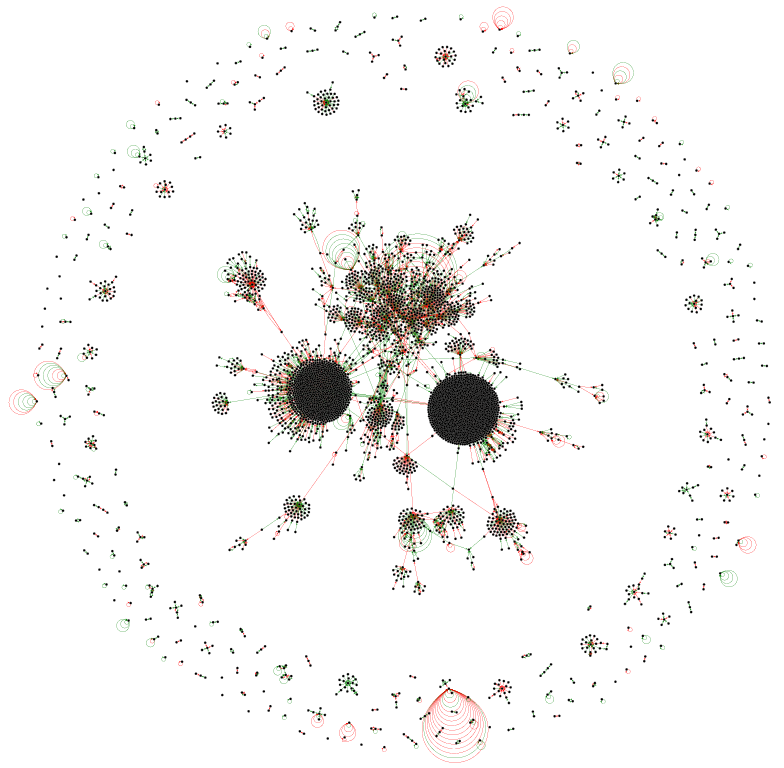
\includegraphics[width=0.8\linewidth]{img/nytimes_20.png}
        % \caption{}%
        \label{fig:img/nytimes_20}
    \end{figure}
% Fraction of nodes in k-core: 1.0
% Fraction of negative edges: 0.4843137254901961
% Clustering coefficient: 0.000817322100229331 with standard deviation 0.0013059816337067929
\end{frame}

\begin{frame}[c]
    \frametitle{A graph on @nytimes (2) - 3-core}
    
    \begin{figure}[htpb]
        \centering
        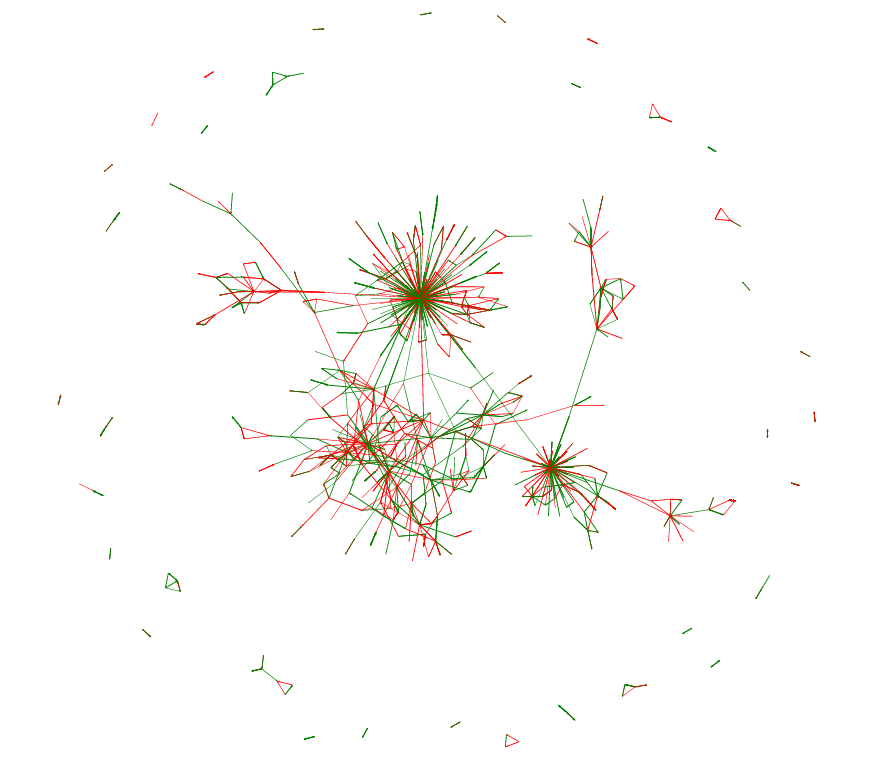
\includegraphics[width=0.8\linewidth]{img/nytimes_20_3.png}
        % \caption{img/Nytimes_20_3}%
        \label{fig:img/nytimes_20_3}
    \end{figure}
\end{frame}

\begin{frame}[c]
    \frametitle{A graph on @nytimes (3) - 3-core}
    \begin{itemize}
        \item The complete graph has 4953 vertices and 6630 edges
        \item The 3-core has 606 vertices and 1955 edges
        \item Fraction of nodes in 3-core: 0.12235009085402786
        \item Fraction of negative edges: 0.4843137254901961
        \item Clustering coefficient: 0.01823698017063645 with standard deviation 0.03642280121409489
    \end{itemize}
\end{frame}

\begin{frame}[c]
    \frametitle{A graph on @FoxNews (1)}
    \begin{figure}[htpb]
        \centering
        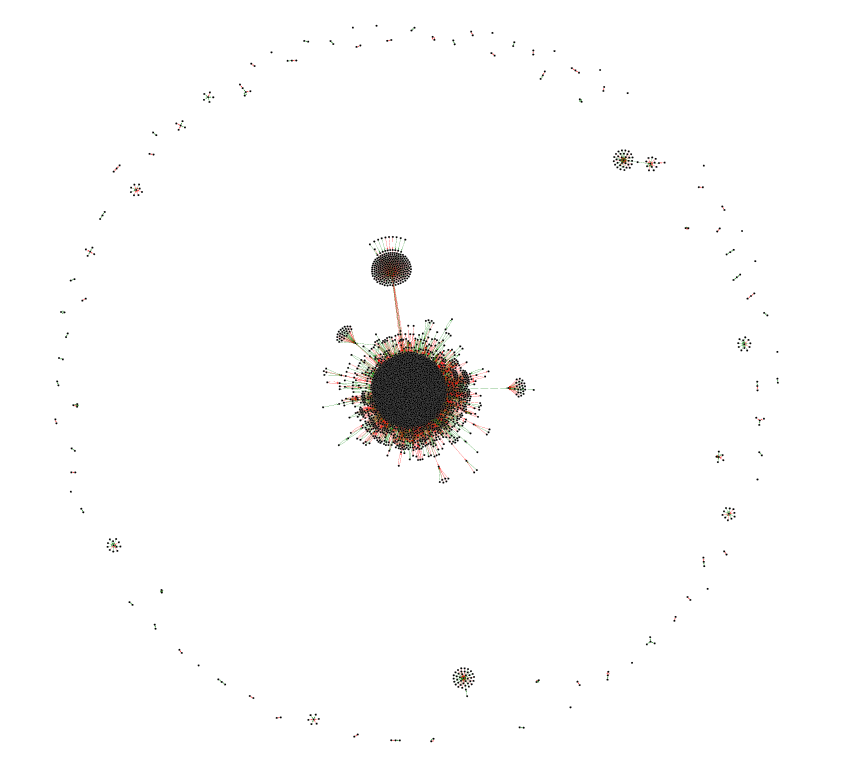
\includegraphics[width=0.8\linewidth]{img/foxnews_20.png}
        % \caption{img/Foxnews_20}%
        \label{fig:img/foxnews_20}
    \end{figure}

    
\end{frame}

% \begin{frame}[c]
%     \frametitle{A graph on @FoxNews (2)}
%     \begin{itemize}
%         \item Fraction of nodes in k-core: 1.0
%         \item Fraction of negative edges: 0.5836486328353552
%         \item Clustering coefficient: 0.00039682210368539454 with standard deviation 0.11713602590613348
%     \end{itemize}
% \end{frame}

\begin{frame}[c]
    \frametitle{A graph on @FoxNews (2) - 3-core}
    \begin{figure}[htpb]
        \centering
        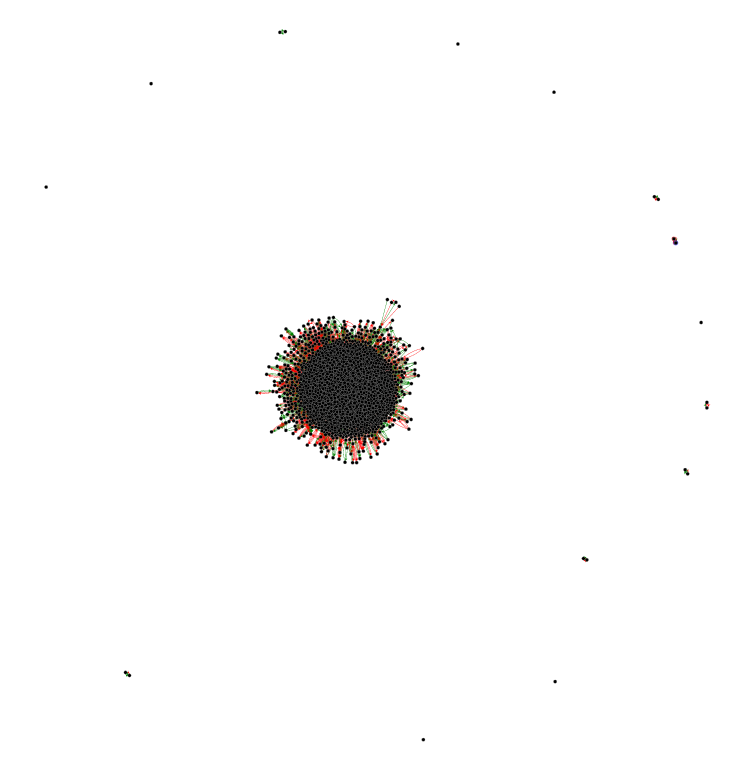
\includegraphics[width=0.8\linewidth]{img/foxnews_20_3.png}
        % \caption{img/Foxnews_20_3}%
        \label{fig:img/foxnews_20_3}
    \end{figure}
\end{frame}

\begin{frame}[c]
    \frametitle{A graph on @FoxNews (3) - 3-core giant component}
    \begin{figure}[htpb]
        \centering
        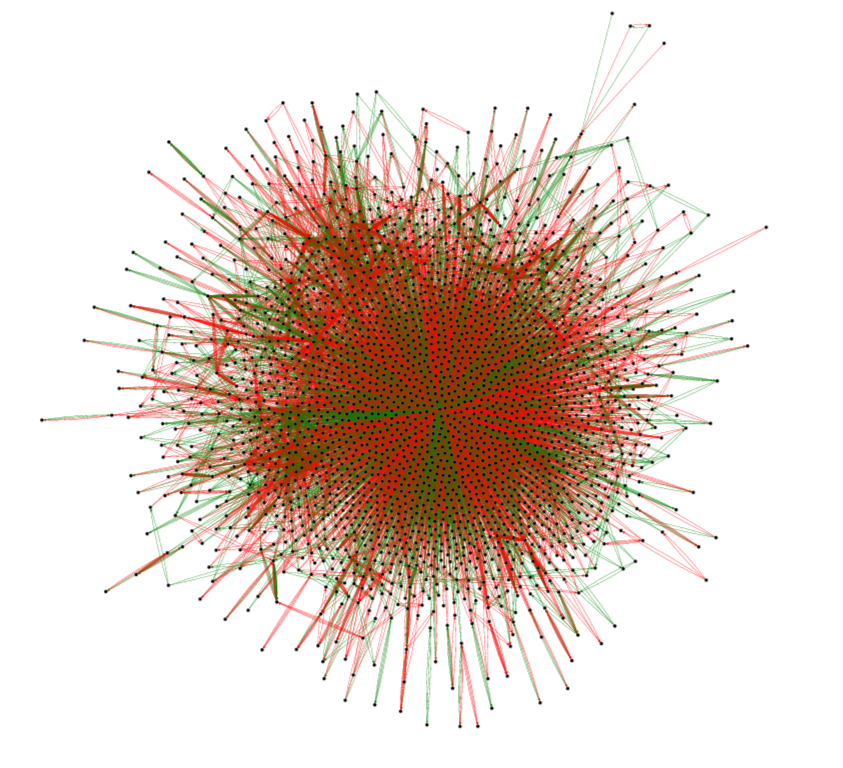
\includegraphics[width=0.8\linewidth]{img/foxnews_20_3_giant.png}
        % \caption{img/Foxnews_20_3}%
        \label{fig:img/foxnews_20_3}
    \end{figure}
\end{frame}

\begin{frame}[c]
    \frametitle{A graph on @FoxNews (4) - 3-core small components}
    \begin{figure}[htpb]
        \centering
        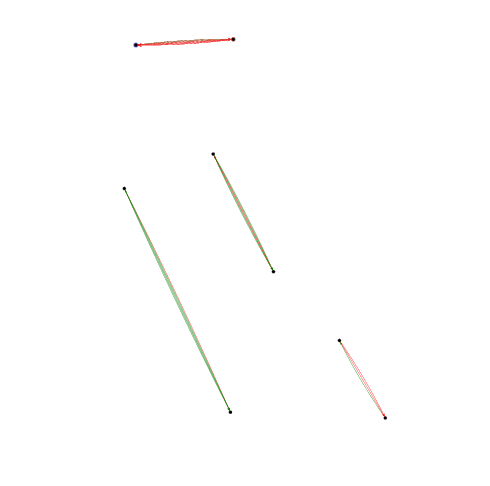
\includegraphics[width=0.8\linewidth]{img/foxnews_20_3_small.png}
        % \caption{img/Foxnews_20_3}%
        \label{fig:img/foxnews_20_3}
    \end{figure}
\end{frame}

\begin{frame}[c]
    \frametitle{A graph on @FoxNews (5) - 3-core}
    \begin{itemize}
        \item The complete graph has 7591 vertices and 25885 edges
        \item The 3-core has 2562 vertices and 16619 edges
        \item Fraction of nodes in 3-core: 0.33750494006059806
        \item Fraction of negative edges: 0.5780567896465134
        \item Clustering coefficient in 3-core: 0.0012715030675363303 with standard deviation 0.14793588681638115
    \end{itemize}    
\end{frame}

% \begin{frame}[c]
%     \frametitle{Next steps}
%     \begin{itemize}
%         \item Comparing different graph with common graph statistics (average
%             shortest path, degree distribution etc.)
%     \end{itemize}
% \end{frame}

\end{document}


